\chapter{PlanetLab Network}
\label{chapter:planetlabnetwork}
PlanetLab is a global research network that enables development of new network services. According to the PlanetLab project main page it was used by more than 1000 researches at top academic institutions and industrial research labs to develop a new technologies for distributed storage, network mapping, peer-to-peer systems, distributed hash tables, and query processing since it launch at 2003 \cite{planetlabmain}. The main page description also states that PlanetLab currently consists of 1353 nodes at 717 sites and their locations worldwide can be seen in Figure~\ref{fig:location}.

\begin{figure}[H]
	\centering
	\scalebox{0.2}{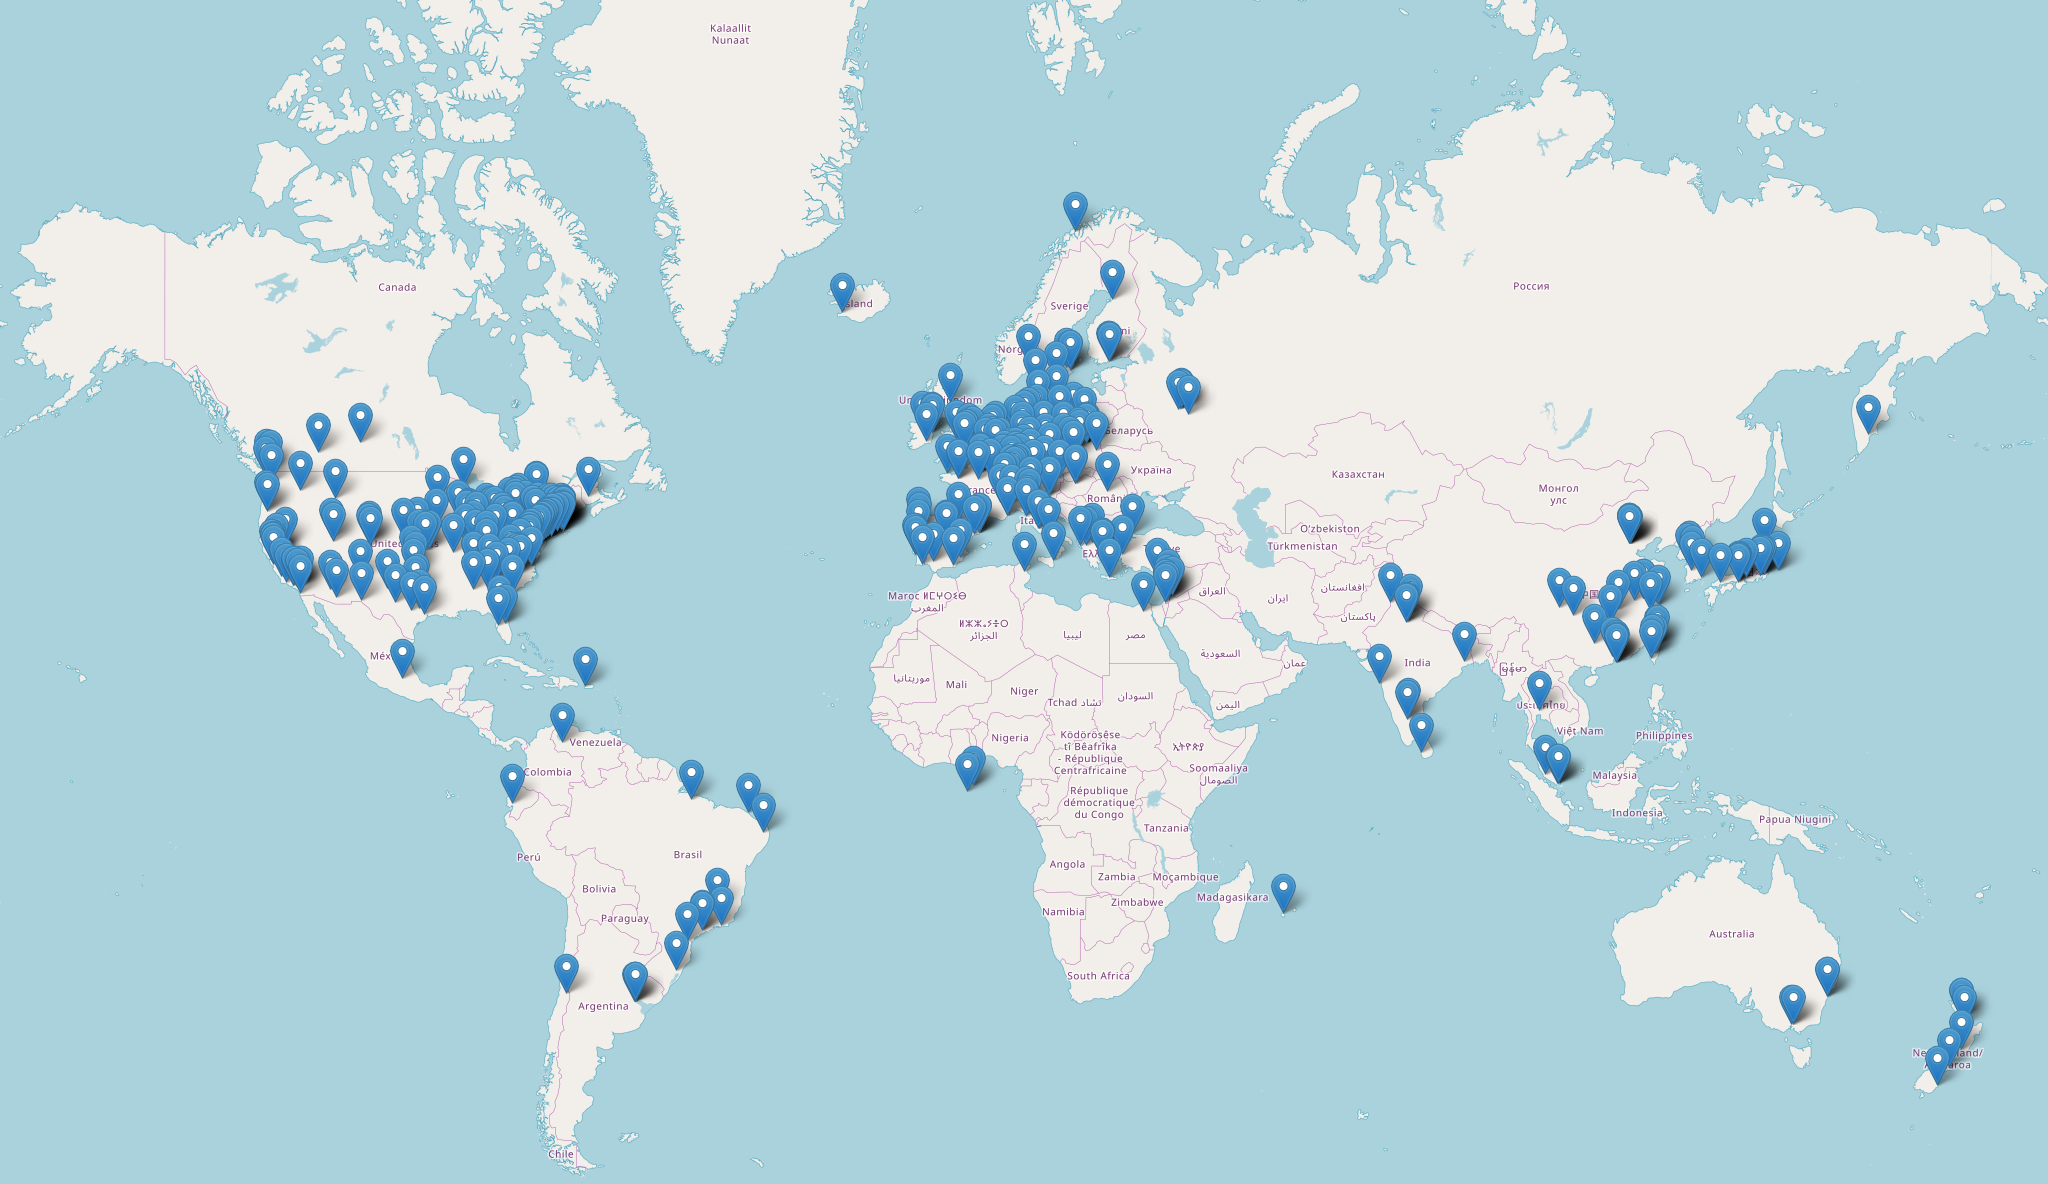
\includegraphics{obrazky/mapa_planetlab}}
	\caption{Map displaying location of the PlanetLab network nodes.}
	\label{fig:location}
\end{figure}

The tool's internal database created using PlanetLab \zk{zkAPI} (\zkratkatext{zkAPI}) consists of 1001 nodes which differs from the number described on the PlanetLab website and is most probably result of removing several nodes since the time website was updated. Important aspect to mention is that not all of those nodes are accessible. As shown in Figure~\ref{fig:pingablepie}, only 196 are responding to \zk{zkICMP} (\zkratkatext{zkICMP}) packets and 805 are not which is only around \SI{19.58}{\percent} reponding nodes. That means \SI{1.62}{\percent} nodes stopped responding since the last measurement done by Filip Šuba in his thesis \cite{suba1} in 2017. Important is to mention that this does not mean that the nodes are not accessible using \texttt{ssh} protocol. The \texttt{plbmng} tool can monitor accessibility of the nodes so its users always has overview which nodes can be actually used for their projects. The current committee of the project consists of members like Princeton University, Cambridge University, Intel, Google and many more \cite{planetlabmain}.\\

\begin{figure}[H]
	\centering
	\scalebox{0.6}{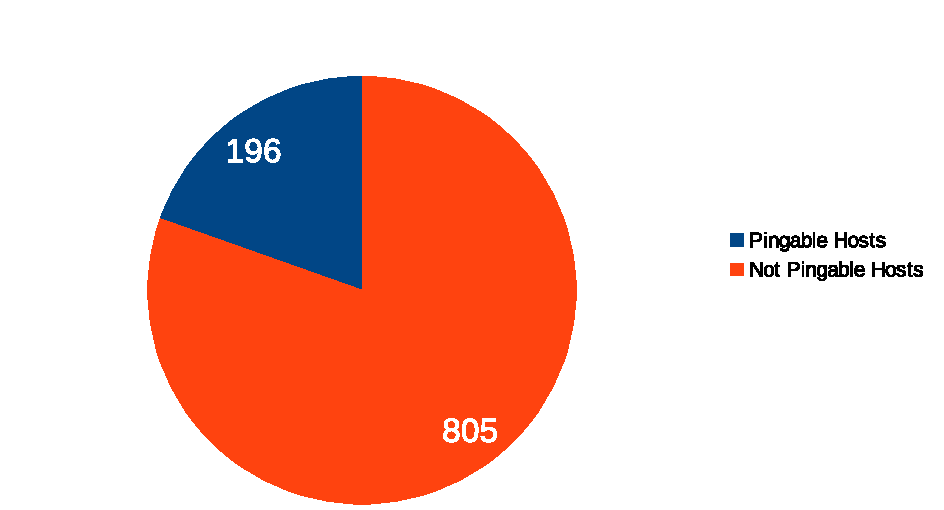
\includegraphics{obrazky/pingablepie}}
	\caption{Pie chart displaying number of nodes in PlanetLab network responding to ICMP packets.}
	\label{fig:pingablepie}
\end{figure}

\section{Use and Terminology}
\label{section:terminology}
During the initial planning of \texttt{PlanetLab network} the authors agreed on using common terminology for aspects of the network and defined them in the \texttt{Phase 0 document} \cite{Roscoe_PDN-02-002} as follows:
\begin{itemize}
	\item \textbf{Node:} A~server machine capable of running components of PlanetLab services.
	\item \textbf{Site:} A~physical geographical location where PlanetLab nodes are located.
	\item \textbf{Cluster:} The set of PlanetLab nodes located at a given site.
	\item \textbf{User:} An authorized human being wishing to deploy or run service over PlanetLab network.
	\item \textbf{Client:} A~client of a service running over PlanetLab network.
	\item \textbf{Service:} An application running over PlanetLab network.
	\item \textbf{Application:} A~PlanetLab service not being part of PlanetLab infrastructure. 
	\item \textbf{Capsule:} A~component of a PlanetLab service that runs on a single node.
	\item \textbf{Slice:} A~distributed set of resources allocated to a service in PlanetLab.
\end{itemize}
\section{Selected Projects Based on PlanetLab}
In this section various projects, that PlanetLab network enabled to create, will be described. All these projects wouldn't be possible without the resources PlanetLab brings. On PlanetLab site there is partial bibliography of research enabled by PlanetLab and it consist of over two hundred projects \cite{planetlabmain}. Having over two hundred projects enabled by PlanetLab network shows that PlanetLab had succeeded in their initial goals which was to provide a useful platform for networking and system research \cite{Roscoe_PDN-02-002}. Example of projects enabled by PlanetLab are described in the following subsections.
\paragraph{Securing Web Service by Automatic Robot Detection}
This project is focusing on detection of automatic robots by implementing a special form of Touring test. Detection is done by comparing human versus robot behavior on the websites. According to the authors, \SI{95}{\percent} of the human users can be detected within the first 57 requests \cite{Park:2006:SWS:1267359.1267382}.
\paragraph{The Design and Implementation of Next Generation Name Service for Internet}
Project that is aiming to solve the vulnerability of the current \zk{zkDNS} (\zkratkatext{zkDNS}) and slow delivery of updates to the system. Project paper describes design and implementation of the Cooperative Domain Name System (CoDoNS), a novel name service, which provides high lookup performance through proactive caching, resilience to denial of service attacks through automatic load-balancing, and fast propagation of updates \cite{Ramasubramanian:2004:DIN:1030194.1015504}.
\paragraph{Slurpie: Cooperative Bulk Data Transfer Protocol}
Big data transfers can become problematic during peaks when huge amount of clients starts downloading the data at one point. This can occur for example during a launch of a new game or a new operating system. Slurpie is is a  a peer-to-peer protocol for bulk data transfer that aims to reduce client download times of large popular files and to reduce load on the providing servers \cite{1356981}. 

\section{PlanetLab Inftrastructure}
\label{section:plinfra}

blabla

\subsection{Operating System Linux}
\label{subsection:Linux}
In this Chapter, the operating system Linux that PlanetLab nodes are running on, and that \texttt{plbmng} tool is developed for, will be reviewed and described. Operating system is a connecting layer between hardware and software. It provides interface to work with system resources such as disk, processor or memory and at the same time it provides service layer for client software to run at. Linux is an open-source operating system founded by Linus Torvalds who wrote its kernel using \texttt{C language} and began the history of Linux operating system. It was originally developed for personal computers based on the Intel x86 architecture but since its creation it has been ported to many other platforms such as mobile devices, television chips and many others. A~package containing Linux operating system is called Linux distribution. The defining component of each distribution is the Linux kernel \cite{eckert2012linux+}. Original Linux kernel has been created by Linus in 1991 \cite{linuxintro} and since then many other forks of this kernel has emerged. Some of the most famous are \texttt{Red Hat Enterprise Linux},  \texttt{CentOS}, \texttt{Fedora}, \texttt{Debian} or \texttt{Ubuntu}. More information about mentioned distributions can be found in at the end of this Chapter. The main advantages of Linux are:
\begin{itemize}
	\item Some Linux distribtuins are free and available for everyone.
	\item Linux is open-sourced and everyone can contribute and review what his/her machine is running.
	\item Linux can run on various platforms from personal computers to televisions.
	\item Linux is considered to be secure. Security model of Linux is based on UNIX security principals which are considered to be robust and verified \cite{BILHEQP2xqVnjbQi}. 
	\item Linux quickly adapt to changes. Since Linux has vast community behind it, it quickly adapt to security threads and new technologies.
\end{itemize}
On other hand, Linux has some disadvantages which are summarized in the below list:
\begin{itemize}
	\item Requires more technical knowledge than other systems like \texttt{Windows} or \texttt{MacOS}.
	\item Huge amount of distributions can be confusing for new users to choose from. 
	\item Many well known applications are primarily developed for \texttt{Windows} or \texttt{MacOS} (though many open source variants of these applications exists on Linux).
	\item Compatibility problems. Proprietary hardware can have issues with driver compatibility. Many hardware vendors are primarily focusing on \texttt{Windows} or \texttt{MacOS}.
\end{itemize}
Linux kernel can be found in majority of devices at the moment. According to StatCounter Global Stats, \SI{41.63}{\percent} of the machines are running on Linux kernel while \SI{36.23}{\percent} are running on Windows-based kernel as of September 2018 \cite{StatCounter}. The rise of Linux kernel is conditioned by raising Android popularity and in 2016 the StatCounter states Linux kernel based system had only \SI{28.44}{\percent} market share while Windows had \SI{48.42}{\percent} market share \cite{StatCounter}. Linux can be found also in great amount of devices from phones, desktops, servers to television or cars. Server \texttt{opensource.com} states that more then half of all SmartTV devices runs on Linux \cite{opensourcecom}. Because Linux kernel is originally open-sourced, most of the devices worldwide runs on an open-sourced operating system which shows an interesting trend switching from proprietary software. In the following paragraphs, various popular Linux distributions will be described and their key features will be reviewed. 
\paragraph{Red Hat Enterprise Linux}
Red Hat Enterprise Linux is a Linux based distribution developed by Red Hat Inc. In 1994 the first version of Red Hat Linux has been released \cite{rhhistory}. Since it launch Red Hat became a popular enterprise Linux distribution and based on Red Hat's June 2017 statistic \SI{100}{\percent} of all airlines, telcos and commercial banks in Fortune 500 runs on their software \cite{rhtrusted}. Red Hat advertise the system being robust and stable which is its biggest advantage for the enterprise companies. Even though Red Hat is open-sourced, it is not free as it is impossible to run it without having active subscription. Red Hat uses its own packaging system called \zk{zkYUM} (\zkratkatext{zkYUM}).
\paragraph{CentOS}
The \zk{zkCENTOS} (\zkratkatext{zkCENTOS}) is a Linux distribution that has been originally forked from Red Hat Enterprise Linux version 2.1 and released under name \texttt{CentOS-2} in May, 2014 \cite{centosfirsts} by John Newbigin. Since then it became a community-driven project that offers and free alternative to the Red Hat Enterprise Linux. Currently, CentOS Project is part of Red Hat while declaring to stay independent of the development of the Red Hat's Linux. Due to the distribution being free while still aiming for enterprise projects, many companies and academic institutions choose the CentOS as the primary operating system for their servers.
\paragraph{Fedora}
Fedora is a Red Hat sponsored Linux distribution developed by the Fedora Project and community around it. Currently, Fedora provides several types of system images such as Workstation for personal computers, Server for servers and Atomic for containerized applications. Fedora is distribution primarily used as a desktop operating system and shares many technologies with Red Hat Enterprise Linux and CentOS making packages compatible between these systems. Fedora is often considered to be a beta environment for changes before they make it to the more conservative Red Hat Enterprise Linux.
\paragraph{Debian}
Originally created in 1993 by Ian Murdock, Debian is a free Linux kernel based Unix like operating system developed by The Debian Project and its community. Debian in oposite to Red Hat Linux based systems uses different packaging system called \zk{zkAPT} (\zkratkatext{zkAPT}). In February 2016 the repositories of Debian consisted of 50007 binary packages \cite{debianfifty}. Debian is popular server distribution and in 2012 it was named by PCWorld magazine the most popular distribution for web servers \cite{debianpopular}.
\paragraph{Ubuntu}
Ubuntu is a free and open-source Linux distribution based on Debian operating system. It is being developed by 	Canonical and Ubuntu community. Currently Ubuntu offers three version of the system: Ubuntu Desktop for personal computers, Ubutnu Server for server and cloud and lastly Ubuntu Atomic created for \zk{zkIOT} (\zkratkatext{zkIOT}). It is seen that Ubuntu makes the Linux more available for broader audience by having its graphical user interface similar to other operating system like \texttt{MacOS}. Ubuntu also achieved great success when Microsoft ported official Ubuntu binaries into its Windows system. Ubuntu is currently the most popular Linux distribution based on Google Trends data \cite{linuxtrends}.
\subsection{Virtualization}
\label{subsection:Virtualization}
Virtualization is an alternative to the traditional architecture. Comparison schema between virtualization and traditional architecture can be found in  Figure~\ref{fig:virtschema}. The traditional architecture consist of a hardware, operating system on the host and the applications running on it. The applications needs to be compatible with the operating system to be able to run on it. On the other hand, virtualization is a layer over the hosting operating system and offers an interface for the guest operating system to use by emulating various resources such as disk, network usb and many more. Guest operating system are operating systems of the virtual hosts running on the hypervisor. Hypervisor is providing resources to each virtual host. This enables better resource handling since all the virtual machines share same resources and theoretically have access to much higher computing power. Another advantage is backward compatibility as various operating systems of a kind can be running one one host. Example is legacy version of a system that is no more compatible with current hardware but is compatible with the virtualization software. This can be particular useful for institutions that requires extremely stable well tested software running on legacy system. Next feature is high availability. If a virtual host crashes, many virtualization software are capable to migrate the run-time data to another virtual host live time. This can be crucial feature for any critical applications. On bare-metal hosts this can be solved by using for example clustered hosts.\\

\begin{figure}[H]
	\centering
	\scalebox{0.7}{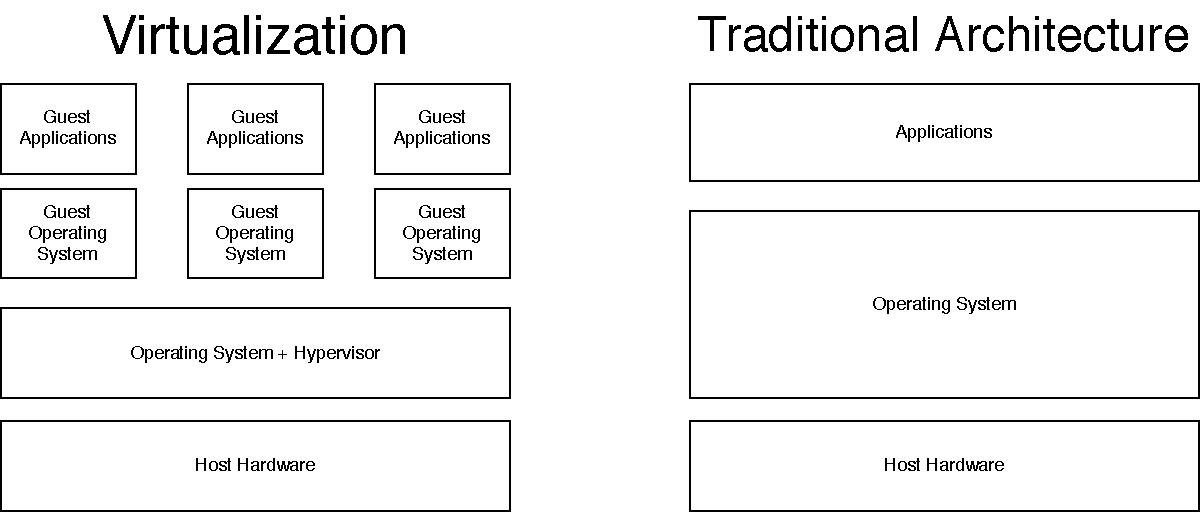
\includegraphics{obrazky/virt}}
	\caption{Virtualization vs traditional architecture schema.}
	\label{fig:virtschema}
\end{figure}

Currently there are many virtualization technologies available on the market. Some of the most popular ones are \texttt{VMware ESXi}, \texttt{Red Hat Enterprise Virtualization}, \texttt{Oracle Virtualbox} and \texttt{QEMU/KVM} \cite{virtualizationpopular}. In the following lines, some of the most popular Virtualization technologies are reviewed.
\paragraph{VMware ESXi}
VMware is a company providing virtualization software. The company provides several versions of virtualization software including \texttt{VMware ESXi} which is an enterprise virtualization solution. \texttt{VMware ESXi} was developed to run directly on the bare-metal hardware and doesn't require any other operating system to be installed on the host as it uses its own operating system called VMkernel \cite{vmwarearch}. This allows the software direct access to the hardware as it includes its own vital OS components. As VMware states in their architecture document \cite{vmwarearch}, this also allows better hypervisor security, increased reliability,
and simplified management. 
\paragraph{Red Hat Enterprise Virtualization}
As Red Hat states on their website, \texttt{Red Hat Enterprise Virtualization} is an open, software-defined platform that virtualizes Linux and Microsoft Windows workloads \cite{rhev}. \texttt{Red Hat Enterprise Virtualization} is a software that is developed to run on Red Hat Enterprise Linux, a Linux distribution developed by the same company. As Red Hat states in \texttt{Red Hat Enterprise Virtualization} datasheet, the biggest advantage of the software is its integration with other \texttt{Red Hat} products \cite{rhdatasheet}. Red Hat also offers a complete operating system designed for creating virtual machines called \texttt{Red Hat Enterprise Virtualization Hypervisor}.
\paragraph{Oracle Virtualbox}
\texttt{Oracle Virtualbox} is open source virtualization software available for both enterprise as well as home use and is developed by Oracle Corporation. As stated on the Oracle Virtualbox website: "Presently, VirtualBox runs on Windows, Linux, Macintosh, and Solaris hosts and supports a large number of guest operating systems including but not limited to Windows (NT 4.0, 2000, XP, Server 2003, Vista, Windows 7, Windows 8, Windows 10), DOS/Windows 3.x, Linux (2.4, 2.6, 3.x and 4.x), Solaris and OpenSolaris, OS/2, and OpenBSD." \cite{oraclehome} which is a considerable availability. \texttt{Oracle Virtualbox} offers many features, which are more described in the User Manual \cite{oracledatasheet}, such as:
\begin{itemize}
	\item VBoxManage, a command-line interface for \texttt{Oracle Virtualbox}.
	\item No hardware virtualization required, supporting even older hardware without build-in virtualization support. 
	\item Guest Additions, which is a software packages that offers features like folder sharing, automatic window focus, 3D virtualization and more.
	\item Multigeneration branched snapshots, which allows taking snapshot of the virtual host in any point of time completely saving the machine state allowing users to later revert machine to the saved state.
\end{itemize}
\paragraph{KVM with QEMU}
\zk{zkKVM} (\zkratkatext{zkKVM}) is a kernel module that provides a \zk{zkCPU} (\zkratkatext{zkCPU}) virtualization through the use of Intel VT or AMD-V hardware extensions. KVM runs in kernel space and handles elements like processor switching or \zk{zkMMU} (\zkratkatext{zkMMU}) registers, which are used to handle the virtual machines. On the other hand, QEMU is a free open source emulator that performs hardware virtualization in the user space part of the operating system. On its own, QEMU provides also CPU emulation through binary translation however the best results are delivered when combined with KVM and it can deliver near native performance \cite{kvmspeed}. During measurement of virtual machine versus host performance using the KVM technology the Geekbench’s GPU test shown only \SI{1.19}{\percent} score decrease over the bare-metal host \cite{kvmbenchmark}.


\chapter{Present State Of Application Development}
\label{chapter:plbmng}
Plbmng application, originally called \texttt{Data miner for PlanetLab}, is a supporting application for developing projects in the PlanetLab network. It gives its user an ability to discover and search PlanetLab servers, connect to them and upload or execute scripts. The tool is available at public PyPI repository\footnote{Link to PyPI repistory containing Data miner for PlanetLab tool: \url{https://pypi.org/project/plbmng/}}. The tool allows managing \texttt{PlanetLab} nodes, gathering information about them and pulling the latest data from the \texttt{PlanetLab} API service. Its core is written in Bash and additional modules are written in Python 3 \cite{suba1}. At the moment, it is depended on both Bash and Python modules and its installation consists of several steps:
\begin{itemize}
	\item Installing the application from PyPI repository or downloading the source codes from GitHub.
	\item Installing additional system packages like dialog,pssh and fping.
	\item Locating installation folder and putting symlink into \texttt{\$PATH} directory.
\end{itemize}
Since improvement of the installation process is in scope of this Diploma thesis, detailed post-improvement installation steps are described later in the Chapter~\ref{chapter:improve}.
\section{Description of Current Functionality}
The tool consist of two layers. First one is the application logic layer and second one is graphical user interface layer, also known as menu, and consists of several options. First menu option is \texttt{Search nodes} for retrieving a node from internal database. This options allows user to either search by \zk{zkDNS} (\zkratkatext{zkDNS}), \zk{zkIP} (\zkratkatext{zkIP}) address or by node location. Second option is \texttt{Measure Menu} that allows user to schedule gathering of data about the nodes using \texttt{crontab}, select elements to monitor or start the data gathering right now. In the \texttt{Map Menu} option user has option to generate map showing location of the nodes and select map element. After the first start of the application, user is required to fill credentials and \texttt{SSH} public key details to be able to access \texttt{PlanetLab} API and nodes using the menu option \texttt{Settings}. Menu is created using bash library \texttt{dialog} and is shown in Figure~\ref{fig:planetlaboldmenu}. Graphical interface can be run directly in terminal making it available even through \texttt{ssh} client without setting up any graphical tools.

\begin{figure}[H]
	\centering
	\scalebox{0.5}{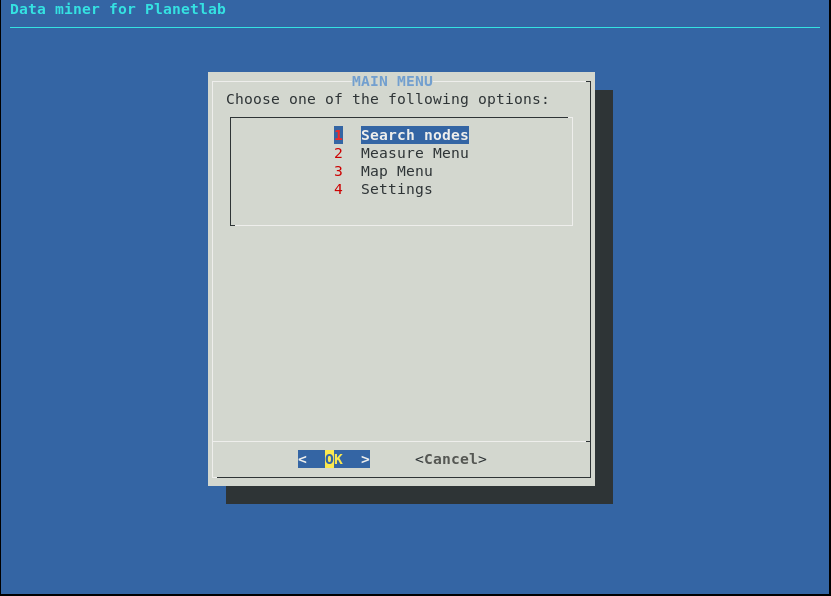
\includegraphics{obrazky/planetlabmenuold}}
	\caption{Menu of previous version called Data miner for PlanetLab.}
	\label{fig:planetlaboldmenu}
\end{figure}


\section{Identified Problems}
\label{section:improvement}
The first problem of the existing tool is language disparity having half of the functionality in Bash and half of the functionality in Python 3. This makes it difficult to make adjustment to the tool as one needs to study a vast amount of scripts that are in several different folders. Since some of the functionality is done in Python 3, which is according to portal StackOverflow fastest-growing major programming language \cite{pythonfastestgrowing}, and because it is available at \zk{zkPYPI} (\zkratkatext{zkPYPI}), Python is an ideal candidate as a main language of the project. As a part of the Diploma thesis the existing code will be re-written into Python 3. Another great advantage of Python 3 is that it is multi-platform. As Mark Pilgrim mentions in his book \cite{Pilgrimc2010}, Python 3 is available on many platform such as \texttt{Windows}, \texttt{MacOS}, \texttt{Linux}, \texttt{BSD} and \texttt{Solaris} and their derivatives.\\
Second area of improvement is installation of the tool and post-installation steps. At the moment, it is required to install additional packages and tool is not automatically put into \texttt{\$PATH} folders forcing its users to locate the installation folder and run the script from there. Because of the single programming language being \texttt{Python 3} the dependencies for system packages will be removed and their \mbox{\texttt{Python 3}} counter-parts will be added as dependency for the PyPI package. PyPI installer takes care of these dependencies automatically during the installation procedure. To remove post-installation steps the tool will be written as library allowing to create a simple \texttt{Python} script in \texttt{bin} folder which is put into \texttt{\$PATH} folder by the PyPI installer during the installation.\\
Another improvement is renaming certain menu components and adding more information to the tool itself. This change is not significant and is purely cosmetic but can make it easier for new users to get familiar with the tool. The specific rename details will be later described in Subsection~\ref{subsection:readability}.\\
The tool currently contains a lot of bugs and bad coding practices. Example of a typical bug is whole application crashing because of missing file when returning back from \texttt{Search nodes} menu. During the rewriting into \texttt{Python 3} there is space to improve certain controls to avoid these crashes and needs to restart the application. As for bad code practices, as an example the tool currently calls functions recursively during returning from child menu page into parent one. This means the previous function menu is stored in the \texttt{stack} waiting for the application to end before released. During rewriting of the tool these implementation details can be changed to stick with the good coding practices. 
